\documentclass{math}

\usepackage{circuitikz}
\usepackage{tikz}

\title{University Physics 2}
\author{Alvin Lin}
\date{January 2018 - May 2018}

\begin{document}

\maketitle

\section*{Circuits}
We will start with a microscopic pictures of current and resistance.
\begin{center}
  \begin{circuitikz}
    \draw (0,0) to[battery, l=\( \Delta V \)] (0,2) -- (4,2)
      to[resistor, l=R] (4,0) -- (0,0);
   \draw[->] (1.5,2.5) -- (2.5,2.5) node[pos=0.5,above] {\( I \)};
  \end{circuitikz}
\end{center}
Current will flow clockwise in this example, from the positive terminal of the
battery through the wires, into the negative terminal. If we look at a small
section of wire at the top.
\begin{center}
  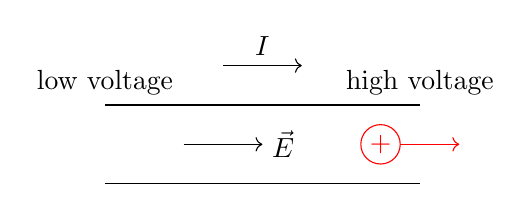
\begin{tikzpicture}
    \draw (0,0) -- (4,0);
    \draw (0,1) node[above] {low voltage} -- (4,1) node[above] {high voltage};
    \draw[->] (1.5,1.5) -- (2.5,1.5) node[pos=0.5,above] {\( I \)};
    \draw[->] (1,0.5) -- (2,0.5) node[right] {\( \vec{E} \)};
    \draw[red] (3.5,0.5) circle (0.25) node[] {+};
    \draw[red,->] (3.75,0.5) -- (4.5,0.5);
  \end{tikzpicture}
\end{center}
We define current, \( I \) as the charge moved through the wire, per unit time.
\[ I = \ddiff{Q}{t} = nqAV_d \]
Sometimes, we will want the current density:
\[ J = \frac{I}{A} = nqV_d \]
All the constants can be defined and rewritten:
\[ \rho = \frac{E}{J} \]
where \( \rho \) is the resistivity of the wire. It is a fundamental property of
a material independent of area or density.
\[ [\rho] = \frac{[E]}{[J]} = \frac{\frac{V}{m}}{\frac{A}{m^2}} =
  \frac{V\cdot m}{A} \]
\begin{align*}
  E &= \rho J \\
  EL &= \rho JL \\
  \Delta V &= \frac{\rho IL}{A} \\
  &= \frac{\rho L}{A}I \\
  R &= \frac{\rho L}{A} \\
  \Delta V &= IR
\end{align*}
This is known as Ohm's Law, where the units of resistance \( R \) are measured
in ohms (\( \Omega \)). All these derivations are done in terms of a positive
charge, but in a wire, the charges that are moving are electrons.
\begin{center}
  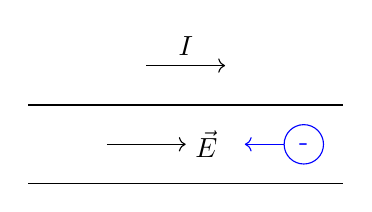
\begin{tikzpicture}
    \draw (0,0) -- (4,0);
    \draw (0,1) -- (4,1);
    \draw[->] (1.5,1.5) -- (2.5,1.5) node[pos=0.5,above] {\( I \)};
    \draw[->] (1,0.5) -- (2,0.5) node[right] {\( \vec{E} \)};
    \draw[blue] (3.5,0.5) circle (0.25) node[] {-};
    \draw[blue,->] (3.25,0.5) -- (2.75,0.5);
  \end{tikzpicture}
\end{center}

\begin{center}
  You can find all my notes at \url{http://omgimanerd.tech/notes}. If you have
  any questions, comments, or concerns, please contact me at
  alvin@omgimanerd.tech
\end{center}

\end{document}
